\subsection{HSQC-TOCSY}
\label{subsec:noah__hsqctocsy}

Having completed our survey of \nitrogen{} modules, we now return to \carbon{} modules: in particular, I was particularly interested in how \textit{two} (or more) modules drawing on \magn{C} magnetisation could be combined in the same supersequence.
Of course, this can be crudely accomplished by simply concatenating two modules which consume all \magn{C} magnetisation: the second of these modules will have greatly reduced sensitivity.
This is acceptable if the second module has a far greater intrinsic sensitivity, but this is not often the case with heteronuclear experiments: thus, a method of \textit{balancing} the sensitivities of the two modules is desirable.
Equivalently, we would like a way to \textit{partition} the magnetisation pool between multiple different modules as we see fit.


\subsubsection{Two HSQC modules}

The strategy used here is in fact a feature of the ASAP-HSQC experiment\autocite{SchulzeSunninghausen2014JACS,SchulzeSunninghausen2017JMR}, previously described in \cref{subsec:poise__asaphsqc}.
In this experiment (which also doubles up as the NOAH HSQC module), the INEPT delay $\DeltaE$ can be changed from its usual value of $1 / (4J)$ (where $J$ is short for $\oneJ{CH}$).
After the \ang{90}($I$)--$\DeltaE$--\ang{180}($I,S$)--$\DeltaE$ INEPT block, the relevant product operators are
\begin{equation}
    \label{eq:inept_changed}
    \cos(2\pi J\DeltaE) I_y - \sin(2\pi J\DeltaE) 2I_xS_z.
\end{equation}
In a `normal' INEPT block, the choice of $\DeltaE = 1/(4J)$ makes the cosine term vanish, leaving us with only the term $-2I_xS_z$.
Since this term is subsequently transferred to spin $S\/$ and labelled in $t_1$, this corresponds to \textit{complete} excitation of \magn{C} magnetisation.

However, if we choose $\DeltaE < 1/(4J)$, then the first $I_y$ term can be `stored' as unexcited \magn{C} magnetisation;
if the remainder of the sequence returns \textit{this} to the $+z$ state, then this portion can be used in a second experiment.
Indeed, this is what happens in the ASAP-HSQC experiment (i.e.\ NOAH HSQC module).
Thus, we could simply construct a \noah{S,S,C} experiment in which the first HSQC module has a suitably modified value of $\DeltaE$: this would achieve the stated aim of partitioning \magn{C} magnetisation between two different modules.
Specifically, in order to excite a fraction $f\/$ of \magn{C} magnetisation (and store the remaining $(1 - f)$ for the next module), we require that
\begin{equation}
    \label{eq:ssc_inept_delay}
    \DeltaE = \frac{2\Delta \arcsin f}{\pi}
\end{equation}
where $\Delta$ is the usual value of $1/(4J)$.
The resulting spectra, obtained by setting $f = 0.8$, are shown in \cref{fig:sscc_example}.


\begin{figure}[!ht]
    \centering
    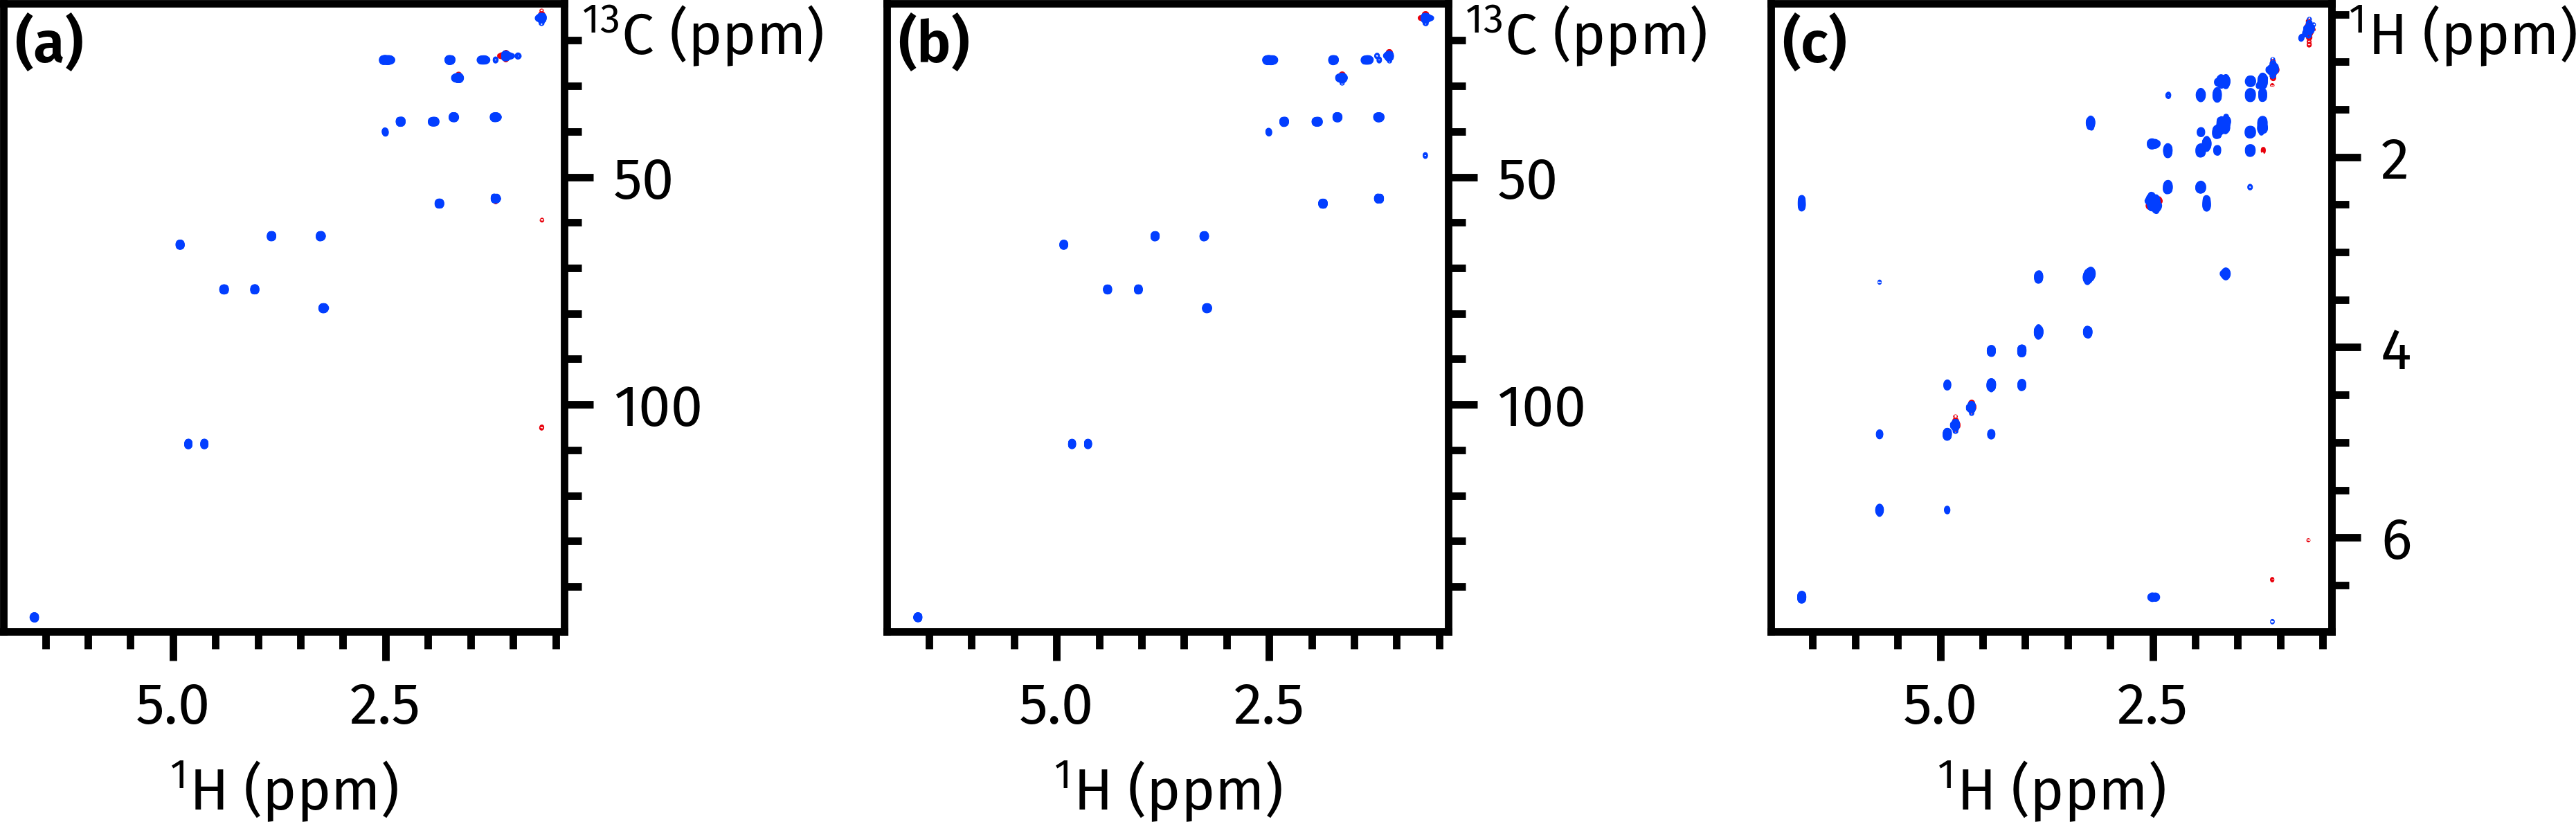
\includegraphics[draft=false]{noah/sscc_example.png}%
    {\phantomsubcaption\label{fig:sscc_example_s1}}%
    {\phantomsubcaption\label{fig:sscc_example_s2}}%
    {\phantomsubcaption\label{fig:sscc_example_cc}}%
    \caption[Spectra from \noah{S,S,Cc} supersequence]{
        Spectra from a \noah{S,S,Cc} supersequence, where the INEPT delay of the first HSQC module was modified to only excite a fraction $f = 0.7$ of \magn{C} magnetisation.
        \textbf{(\subref*{fig:sscc_example_s1})} First HSQC.
        \textbf{(\subref*{fig:sscc_example_s2})} Second HSQC.
        \textbf{(\subref*{fig:sscc_example_cc})} CLIP-COSY.
        \datacode{7A-201010}
    }
    \label{fig:sscc_example}
\end{figure}

In \cref{fig:sscc_improvements_base}, the intensities of these spectra are compared against the HSQC and CLIP-COSY in a \noah{S,Cc} supersequence.
As expected, the first HSQC has 80\% of its sensitivity.
However, the second HSQC spectrum has around 65\% of this `base' sensitivity, despite only nominally having 20\% of the \magn{C} magnetisation to work with.
This is largely due to \magn{C} magnetisation which recovers during the FID of the first HSQC.
Since both HSQC modules do not perfectly preserve \magnnot{C} magnetisation, the CLIP-COSY experiences a very small sensitivity loss (compared to a \noah{S,Cc} supersequence where only one HSQC module is used, which in turn is slightly less sensitive than a standalone CLIP-COSY).

\begin{figure}[!ht]
    \centering
    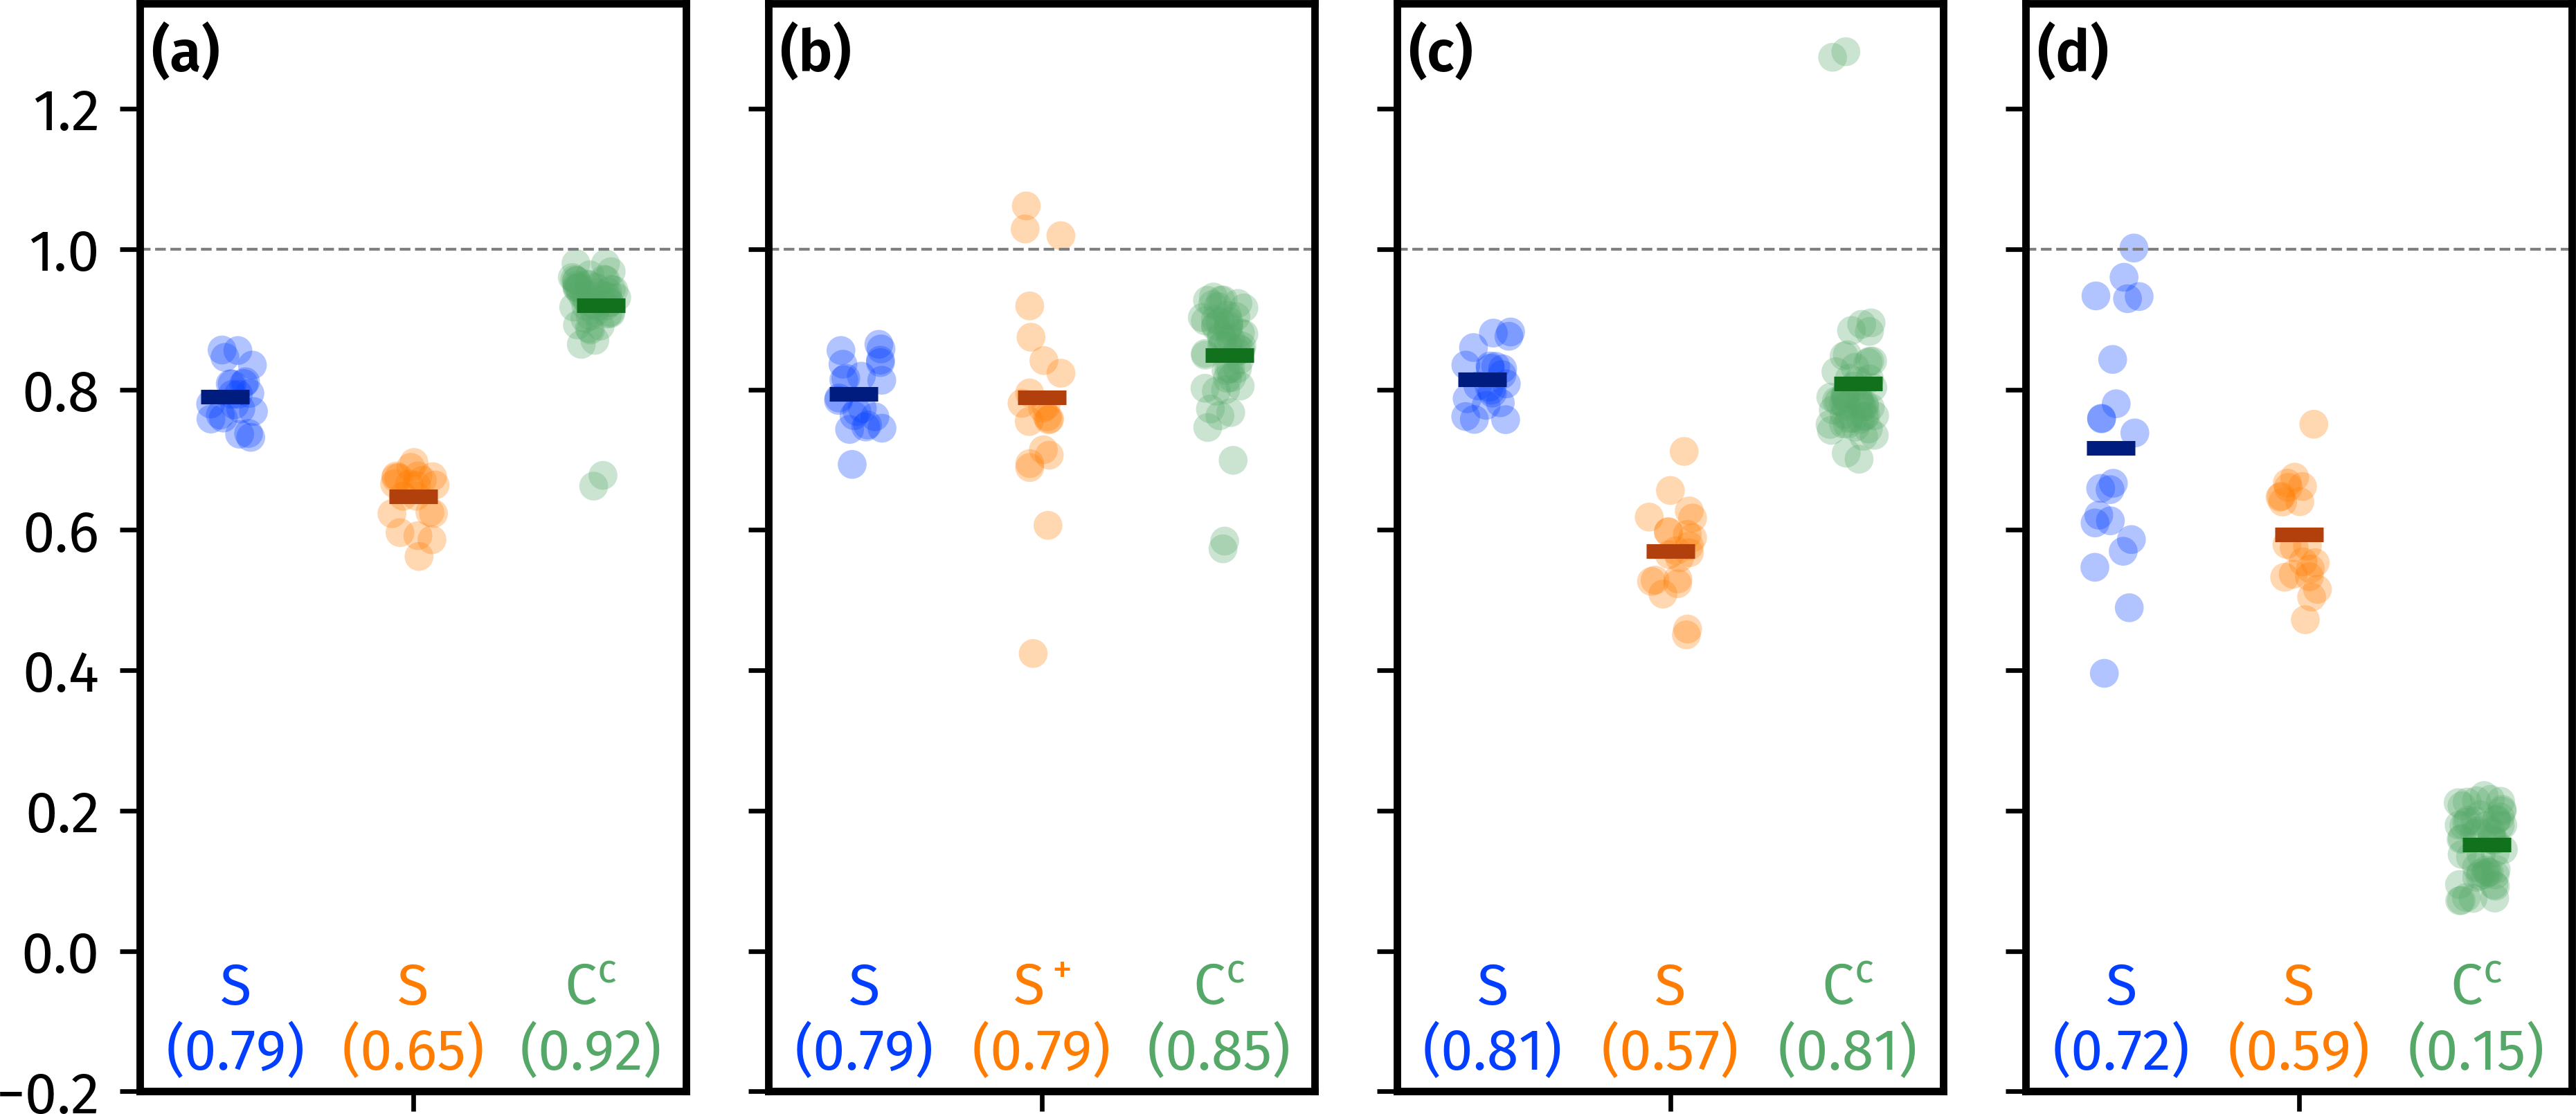
\includegraphics[draft=false]{noah/sscc_improvements.png}%
    {\phantomsubcaption\label{fig:sscc_improvements_base}}%
    {\phantomsubcaption\label{fig:sscc_improvements_sehsqc}}%
    {\phantomsubcaption\label{fig:sscc_improvements_dipsi}}%
    {\phantomsubcaption\label{fig:sscc_improvements_mfa}}%
    \caption[Sensitivity comparisons for \noah{S,S,Cc} and \noah{S,Sp,Cc} supersequences]{
        Comparisons of HSQC and CLIP-COSY sensitivities of \noah{S,S,Cc} and \noah*{S,Sp,Cc} supersequences.
        The fraction of \magn{C} magnetisation excited in the first module, $f$, is set to $0.8$.
        Peak intensities are normalised against the HSQC and CLIP-COSY experiments in a \noah{S,Cc} supersequence.
        \textbf{(\subref*{fig:sscc_improvements_base})} \noah{S,S,Cc} (the same spectra as shown in \cref{fig:sscc_example}).
        \textbf{(\subref*{fig:sscc_improvements_sehsqc})} \noah{S,Sp,Cc}.
        \textbf{(\subref*{fig:sscc_improvements_dipsi})} \noah{S,S,Cc} with \qty{35}{\ms} DIPSI-2 mixing after the first HSQC module.
        \textbf{(\subref*{fig:sscc_improvements_mfa})} A \noah{S,S,Cc} supersequence, but using the seHSQC-splitting implementation of Nolis et al.\autocite{Nolis2019CPC} (as opposed to the ASAP-HSQC module) for the double HSQC.
    }
    \label{fig:sscc_improvements}
\end{figure}

The sensitivity of the second HSQC module can be further improved by simply using the seHSQC module (specifically, the seHSQC2) in place of it.
The effects of this are shown in \cref{fig:sscc_improvements_sehsqc}: sensitivity improvements are obtained in that module itself (although they are not uniform as they depend on multiplicity), and the CLIP-COSY sensitivity is decreased slightly due to poorer \magnnot{C} preservation.
These are entirely in line with the previous discussion in \cref{subsec:noah__sehsqc_c}.

It is also possible to include a period of isotropic mixing between the two HSQC modules: here, the DIPSI-2 sequence\autocite{Shaka1988JMR} was chosen.
Since the \magn{C} magnetisation pool has been (partially) depleted, and the \magnnot{C} magnetisation pool is (almost) full, this should in theory lead to transfer of polarisation from the \magnnot{C} pool to \magn{C}.
However, when tested, this was not found to have a beneficial impact on the supersequence sensitivity (\cref{fig:sscc_improvements_dipsi}): in fact, 
One caveat is that this leads to slightly uneven intensities: since DIPSI transfers magnetisation through scalar couplings, peaks corresponding to protons with fewer coupling partners experience smaller gains in intensity.

\todo{Pulse sequence with prod ops??}

\todo{Multiplicity editing --- not properly implemented in GENESIS?!}


On its own, the acquisition of two HSQC spectra---as has so far been shown---is not particularly interesting.
However, it is possible to differentiate the two HSQC signals and thereby extract more information.
For example, one spectrum may be run without decoupling in order to measure one-bond coupling constants\autocite{Enthart2008JMR,Nolis2019CPC}; or the indirect-dimension spectral width of one of the HSQC spectra can be changed in order to make use of spectral aliasing techniques\autocite{Nolis2019JMR,Jeannerat2011eMR}.
The pulse sequence itself may also be modified: for example, the addition of an isotropic mixing block to the first HSQC yields a HSQC-TOCSY + HSQC combination\autocite{Nolis2019CPC}, which I now discuss.


\subsubsection{HSQC-TOCSY}

The addition of DIPSI mixing
This in fact leads to the ASAP-HSQC-TOCSY experiment, also previously reported by Luy and coworkers\autocite{Becker2019JMR}.

